% 第 4 题伪代码框（全库首例「代码框」图元）：按固定源 PDF 内容流实测值换算（1 bp → 0.03515 cm）。
% 原点取框左下角（源页 (182.52, 484.75) pdf 坐标），y 向上。
% 源为 LaTeX tabular |l| 带边框排布：上下各 1 条通长横线（82.26 pt）；
% 左右竖线各分 7 段（每段恰一行高 15.12 pt，段间 0.12 pt 接缝，1200 dpi 不可见，照源分段）。
% 框内 7 行文本：第 1/2/3/6/7 行左缩进 6 pt（tabcolsep），第 4/5 行再缩进 2 em（21 pt）；
% 字体照源：S、I 为数学斜体（CMMI），← 为 \leftarrow（CMSY），While/End/Print 为正体，数字与 + 为 CMR。
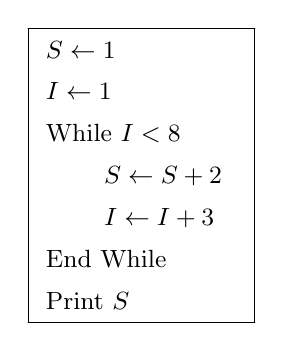
\begin{tikzpicture}[line cap=round,line join=round,font=\small,x=0.03515cm,y=0.03515cm]
% ===== 边框（上下横线 2 条 + 左右竖线 7 段 ×2）=====
\draw (0,0)--(81.86,0);  % 下横线
\draw (0,106.24)--(81.86,106.24);  % 上横线
\draw (0,106.04)--(0,90.92);  % 左竖线第 1 段
\draw (0,90.92)--(0,75.8);  % 左竖线第 2 段
\draw (0,75.8)--(0,60.68);  % 左竖线第 3 段
\draw (0,60.68)--(0,45.56);  % 左竖线第 4 段
\draw (0,45.56)--(0,30.44);  % 左竖线第 5 段
\draw (0,30.44)--(0,15.32);  % 左竖线第 6 段
\draw (0,15.32)--(0,0.2);  % 左竖线第 7 段
\draw (81.86,106.04)--(81.86,90.92);  % 右竖线第 1 段
\draw (81.86,90.92)--(81.86,75.8);  % 右竖线第 2 段
\draw (81.86,75.8)--(81.86,60.68);  % 右竖线第 3 段
\draw (81.86,60.68)--(81.86,45.56);  % 右竖线第 4 段
\draw (81.86,45.56)--(81.86,30.44);  % 右竖线第 5 段
\draw (81.86,30.44)--(81.86,15.32);  % 右竖线第 6 段
\draw (81.86,15.32)--(81.86,0.2);  % 右竖线第 7 段
% ===== 框内 7 行文本（照源基线左端）=====
\node[anchor=base west,inner sep=0] at (6.18,95.458) {\(S\leftarrow 1\)};
\node[anchor=base west,inner sep=0] at (6.18,80.338) {\(I\leftarrow 1\)};
\node[anchor=base west,inner sep=0] at (6.18,65.218) {While \(I<8\)};
\node[anchor=base west,inner sep=0] at (27.18,50.098) {\(S\leftarrow S+2\)};
\node[anchor=base west,inner sep=0] at (27.18,34.978) {\(I\leftarrow I+3\)};
\node[anchor=base west,inner sep=0] at (6.18,19.858) {End While};
\node[anchor=base west,inner sep=0] at (6.18,4.738) {Print \(S\)};
\end{tikzpicture}
